\subsection{Development process, methodology and work flow}

We started on this project as part of a course work for TDT4290---Customer Driven Project. In this project, we have been able to walk through the processes of software development efforts an average software engineer would have gone through in an industrial setting. We have tried to keep the feel and the work as standard as possible and replicated software development processes as properly as we can. This gave us an invaluable insight into how we handle, schedule, manage, trace and carry out tasks in software development projects and below is an evaluation of our experience in this project.
	\subsubsection{Development methodology---Scrum}

With scrum being the most popular software development methodology these days plus the fact that all the team members had some sort of experience with it---which helped save a considerable amount of time we would have spent learning the basics of scrum---and that, among other things, scrum enables to break down tasks into several manageable chunks made scrum an ideal methodology to employ in our project as well. Adopting pure scrum seemed rather less optimistic since all team members had responsibilities in other courses with demanding projects and attending five days of stand up meeting consistently by all groups looked unrealistic. Scrum is also complex administrative wise and team members might also be lost in all the updating and stand-up meetings. And since we started this project in order to develop a prototype, scrum made it easy to revise requirements, implementations and features in constant and periodical contact with our customer.

To make sure such things went smoothly, we had to get together early and decide on how we follow scrum and made amends that suited all members. we decided to hold a stand-up meeting---a time slot when everyone will be able to inform other members of self-completed task and plan for the day ahead---to keep everyone abreast of changes in the the development project. We also fixed sprint lengths to maximum of two weeks. This arrangement has been so effective we had negligible problems. One of the challenging thing to do associated with our scrum was to get something done on each day, to wake up early and show up every Monday to Thursday morning at 9 to relate our work. Some group members work late into the night and making it early in the morning was a bit of an inconvenience but we decided to stick to the plan and that has helped us complete a greater portion of requirements gathering and analysis task early for approval with our customer. We did not employ a post it note row as part of our sprint work backlog. we rather depended on oral communication and everyone took the responsibility of completing missing parts depending on the stand-up meetings every morning. At times, we had to explicitly assign tasks if we felt that some unpopular tasks were being bounced around. In general, the flexible division of work, the consistent stand-up meeting, and the minimum threshold we set for asking questions together with the team members familiarity with scrum has made our work relatively trouble free.
	\subsubsection{Implementation}
The implementation would have been simpler and perhaps faster had it been an application that was going to be deployed on either Android or iOS platforms as native application.
But the requirement was that the application should have one code base and run on both platforms.
It is a cross-platform application.
None of us had any experience with that sort of thing, so the natural thing to do was to make sure every one of us evaluated some framework for the implementation of the requirement.
A number of frameworks came on the table and we had to weigh one against another.
We selected the relatively new PhoneGap for many reasons, as specified in detail in earlier sections of this project document.
Learning the new framework, getting to know existing API's from our customer and on how we were going to integrate our solutions to the customer requirements provided its own challenges.
And we also wanted to develop an application that not only did the functionalities but also have some elegant interface which is less confusing and appealing to end users.

The use of PhoneGap in collaboration with JQuery Mobile made the design of our UI very simple and gave us additional time for shaping the application itself.
Our customer also provided us with a style-sheet used in their online touch device portal so that the designs would match.
Although being a great framework for our purpose, PhoneGap also had it's shortcoming.
Because it's a script-language run in the web-application of the mobile device it's performance is limited compared to a standalone native app.
This downside is also observable in our app, the responsiveness and page transitions are noticeably slower than what would've been the case for a native app.
However we believe this is within reasonable limits and further improvements could possibly make it faster.

The implementation took place in line with our requirements elicitation, working first on the highest priority and starting early on high complexity requirements.
The implementation needed a collaboration between the group members who were investing so much effort on the codes and we used GitHub for listing issues and tracing changes.

In general, we had exactly 10 requirements of which four were high priority and one with high complexity.
Nine of the ten requirements were successfully implemented according to the customer's requirements.
The final requirement was quite complex and also goes against mobile app conventions so it wasn't feasible to implement within our scheduled time. (TODO refer to where this is discussed)

	\subsubsection{Time estimation}
	This project lasted from week 35 until week 47. During this period introduction, project planning and preliminary study took 3 weeks of time, sprint zero 1 week and sprints one-four 2 weeks each. Documentation was written throughout whole period, while last 3 weeks were dedicated only for finishing remaining sections and revision of whole document.\newline
	Members had short stand-up meetings every day Monday - Thursday at 9:15. After internal group evaluation (week 8 of this project) additional teem meeting is determined for Mondays after stand-up meetings. Most working hours were earned in first days of the week, and most work load for this project was on first few weeks and last month.\newline	
	Each week average time spent for advisor, customer and internal meetings was 2 hours. Lectures took average of 2 hours per week for whole project.
	
	TODO SOMETHING ABOUT WORKING HOURS, SOME GRAPH ETC...

    \begin{figure}[htb]
        \centering
        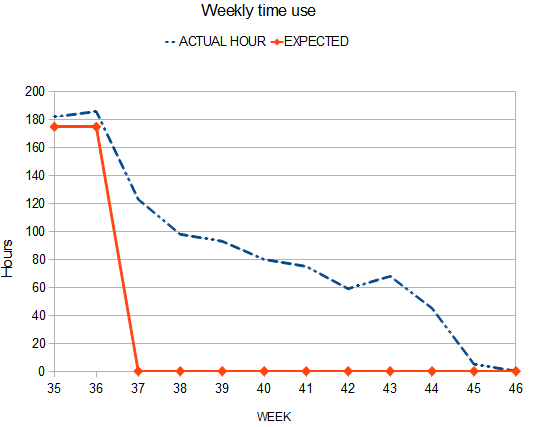
\includegraphics[scale=0.88]{timebudget.png}
        \label{fig:time}
    \end{figure}
	
	\subsubsection{Seminars and study process}
	To make this project better,  the team attended a lot of seminars organized by IDI for this course. This lectures and practical exercises were very important for better understanding of the given problem, better communication between team members, and easier project work flow. Some of the most important seminars were:
	
	\subparagraph{Group dynamics} - one of the first and maybe most important seminar showed values of good team work and importance of correct communication inside the team. It helped people in group to understand mutual differences and to achieve better communication without knowing other persons before. Also, it was nicely explained how team work should lead to better efficiency and more productivity, and it is always good to hear something about that from experienced people working with big groups for a long time.
	\subparagraph{Project management} - one of the less known thing for not experienced students is to manage big projects like this one. In this seminar team listened about how project should be defined, what are goals and objectives and what are starting points for development process. Some points about time estimation and planning for project phases was useful to hear and partly used with this project also.
	\subparagraph{Scrum, an agile development method} - mostly all of the team members was already familiar with scrum development process. Considering scrum as one of the most used method for developing software in past years, everyone had basic knowledge about it. Also, at the very beginning of this project team had several discusses about choice between scrum and waterfall model, so this seminar came little late for any major change in our plan. Although, it was nice to get some deeper knowledge about development method that is already selected.
	\subparagraph{Technical writing} - very useful interactive presentation given by prof. Nancy Lea Eik-Ness. It came after preliminary delivery of project report, which was very good because teams could understand their own disadvantages. During this seminar some part of this report are written, and later improved and included. Also, commented version of our report was very encouraging and confirmed that what we have been doing was not so bad.
	\subparagraph{Presentation techniques} - one of the thing important for making customer satisfied is presentation of finished project. This seminar held by presenter with great experience from Statoil was really interesting and helpful. Most of the team members didn't have much experience with presenting their project to real customer, so this instructive tutorial must be of great help for all.

It seems rather difficult to describe the seminars in such a short paragraph and each group member had an opinion. But everyone seems to have at least found the presentation technique seminar either enjoyable or useful for our project.


